\documentclass[11pt]{article} % DO NOT CHANGE THIS
\usepackage{deauthor}
\usepackage{natbib}
\usepackage{hyperref}  
\usepackage{graphicx}  % hyperlinks
\usepackage{url} 
\usepackage{xcolor}
\usepackage{wrapfig}% simple URL typesetting
\usepackage{booktabs}       % professional-quality tables
\usepackage{amsfonts}       % blackboard math symbols
\usepackage{nicefrac}       % compact symbols for 1/2, etc.
\usepackage{microtype}      % microtypography

\usepackage{microtype}
\usepackage{amsmath}
\usepackage{algpseudocode}
\usepackage{algorithm}
\usepackage{multirow}
\usepackage{subcaption}
\usepackage{bm}
\usepackage{stfloats}
\usepackage{arydshln}
%\usepackage{inconsolata}
\usepackage{graphicx}  
\usepackage{comment}
\usepackage{enumitem}

\newcommand{\ie}{\textit{i.e.}}
\newcommand{\eg}{\textit{e.g.}}
\setcounter{secnumdepth}{2} %May be changed to 1 or 2 if section numbers are desired.

\begin{document}

\title{\textsc{ReFIT}: Reranker Relevance Feedback during Inference}
\pagestyle{plain}
\author{\textbf{Revanth Gangi Reddy}$^1$ \hspace{0.2em} \textbf{Pradeep Dasigi}$^2$ \hspace{0.2em} \textbf{Md Arafat Sultan}$^3$ \hspace{0.2em} \textbf{Arman Cohan}$^{2,4}$ \\ \textbf{Avirup Sil}$^3$ \hspace{0.2em} \textbf{Heng Ji}$^1$ \hspace{0.2em} \textbf{Hannaneh Hajishirzi}$^{2,5}$ \\
$^1$University of Illinois at Urbana-Champaign \hspace{0.5em}  $^2$Allen Institute for AI \\ $^3$IBM Research AI \hspace{0.5em} $^4$Yale University \hspace{0.2em} $^5$University of Washington\\
  \texttt{\{revanth3,hengji\}@illinois.edu} \hspace{0.4em} \texttt{\{pradeepd,armanc,hannah\}@allenai.org} \\
  \texttt{arafat.sultan@ibm.com}\hspace{0.4em} \texttt{avi@us.ibm.com}
  }
\maketitle

\begin{abstract}

Retrieve-and-rerank is a prevalent framework in neural information retrieval, wherein a bi-encoder network initially retrieves a pre-defined number of candidates (\eg{}, $K$=100), which are then reranked by a more powerful cross-encoder model. While the reranker often yields improved candidate scores compared to the retriever, its scope is confined to only the top $K$ retrieved candidates. As a result, the reranker cannot improve retrieval performance in terms of Recall@K. In this work, we propose to leverage the reranker to improve recall by making it provide relevance feedback to the retriever at \textit{inference-time}. Specifically, given a test instance during inference, we distill the reranker's predictions for that instance into the retriever's query representation using a lightweight update mechanism. The aim of the distillation loss is to align the retriever's candidate scores more closely with those produced by the reranker. The algorithm then proceeds by executing a second retrieval step using the updated query vector. We empirically demonstrate that this method, applicable to various retrieve-and-rerank frameworks, substantially enhances the retrieval recall across multiple domains, languages, and modalities.

\end{abstract}

\section{Introduction}
\label{sec:intro}

Federated Learning (FL) is a distributed machine learning (ML) paradigm that trains a model across a number of participating entities holding local data samples.
% , without exchanging them. 
In this work, we focus on \emph{cross-device} FL that harnesses a large number (up to hundreds of millions) of edge devices with disparate characteristics such as availability, compute, memory, or connectivity
resources~\citep{kairouz2019advances}. %that harnesses potential
% Current applications of FL are designed to scale up to client populations of hundreds of millions or even billions. 
Two challenges to the success of cross-device FL are privacy and scalability. 
FL was originally motivated for improving privacy since data points remain on client devices. 
% and only small model updates were shared to a co-ordinating server.
However, as with other forms of ML, information about training data can be extracted via membership inference or reconstruction attacks on a trained model \citep{carlini2021membership,carlini2020extracting}, or leaked through local updates~\citep{MelisSCS19,geiping2020inverting}. 
Consequently, Secure Aggregation (\SecAgg) protocols were introduced to prevent the server from directly observing individual client updates, which is a major vector for information leakage~\citep{bonavitz2019federated,huba2021papaya}. 
Additional mitigations such as  Differential Privacy (DP) may be required to offer further protection 
against attacks~\citep{dwork2006calibrating,abadi2016deep}, as discussed in Section~\ref{sec:discussion}.
% , as discussed in Section~\ref{sec:discussion}.
%As an additional layer of protection against statistical inference attacks, SecAgg is usually paired with Differential Privacy (DP) \citep{dwork2006calibrating}. To realize the full promise of FL as a privacy-enhancing technology, we need both SecAgg and Differential Privacy.

Ensuring scalability to populations of heterogeneous clients is the second challenge for FL.
% There are many aspects for FL scalability, such as ensuring that model updates can be calculated efficiently 
% by devices with various capabilities and intermittent availability~\citep{bonavitz2019federated}.
% Here, we focus on the communication bottleneck as the primary concern.
Indeed, wall-clock training times are highly correlated with increasing model and batch sizes~\citep{huba2021papaya}, even with recent efforts such as FedBuff~\citep{nguyen2021federated},
% With increasing model and batch sizes, the wall-clock training time increases accordingly~\citep{huba2021papaya}. 
% Despite efforts such as buffered asynchronous aggregation~\cite{nguyen2021federated}, 
and communication overhead between the server and clients dominates model convergence time.
% cross-device FL remains bottlenecked by communication latency between the server and the clients. 
% \karthik{should we mention this paper in a different way? Fedbuff paper doesn't explicitly call out latency as an issue, nor do we run experiments to on async fl ourselves}  \ashkan{I also think the transition can be smoother: first we focus on scalability and billions. Then we say communication is the bottleneck} 
Consequently, compression techniques were used to reduce the communication bandwidth while maintaining model accuracy.
However, a fundamental problem has been largely overlooked in the literature: in their native form, standard compression methods such as scalar quantization and pruning are not compatible with \SecAgg. 
This makes it challenging to ensure both security and communication efficiency.
% at the same time.
% the default method to provide security for client update, 
% presenting an unpleasant dichotomy between security or efficiency. 


% Second, this is the most restricted direction, since upload bandwidth remains more restricted than download. 
% In the US, fixed-line broadband speeds typically achieve a ratio of $3\times$ to $20\times$ more download bandwidth than upload
% bottlenecks remain, and so we seek to reduce the message size of clients by \textit{compression}. 
% Compression has been widely proposed in various ML scenarios, in the form of pruning (removing model parameters) and quantization (reducing fidelity of parameter representation). 
% Indeed, these techniques have been successfully used in FL settings with appreciable improvements in communication while maintaining model accuracy. 
% However, there is a fundamental problem which has been largely overlooked in the literature: in their native form, these compression methods are not compatible with SecAgg, the default method to provide security for client updates. 
% This presents an unpleasant dichotomy: we can have security or efficiency, but not both. 
%
%
% In this paper, we resolve this gap by showing how to modify FL compression techniques to make them security-friendly. We focus on compressing \emph{uplink} updates from clients to the server for two reasons. 
% First, uplink communications are subject to Secure Aggregation protocols to ensure a high security bar, while downlink updates broadcasted by the server are deemed public. 
% Second, upload bandwidth is generally more restricted than download. For instance, according to the most recent FCC report, the ratio of download to upload speeds for DSL/cable providers\footnote{Fixed-line broadband is most relevant since FL is typically restricted to using unmetered connections, usually over Wi-Fi~\citep{huba2021papaya}.} in the US ranges between 3$\times$ to 20$\times$~\citep{fcc-broadband}.
% % This requires some meticulous changes to coordinate clients to use the same global (non-private) hyperparameters, and show that this coordination does not damage model quality. 
% % For the strongest compression methods, we step outside of the SecAgg primitive and propose a new secure primitive, Secure Indexing, which enables the best compression ratios without sacrificing utility. 
% Finally, efficient and secure uplink communication brings several benefits beyond speeding up convergence: 
% lowering communication cost reduces selection bias due to undersampling clients with limited connectivity, improving fairness and inclusivity metrics. 
% It also shrinks the carbon footprint of FL, whose fraction attributable to communication can reach 95\%~\citep{qiu2021first}.
%
%In this paper, w
We address this gap by adapting compression techniques to make them compatible with \SecAgg. We focus on compressing \emph{uplink} updates from clients to the server for three reasons. 
First, uplink communication is more sensitive and so is subject to a high security bar, whereas downlink updates broadcast by the server are deemed public. 
Second, upload bandwidth is generally more restricted than download bandwidth. For instance, according to 
a recent FCC report, 
%the most recent \modif{FCC\footnote{\modif{US Federal Communications Commission.}} report}, 
the ratio of download to upload speeds for DSL and cable providers\footnote{FL is typically restricted to using unmetered connections, usually over Wi-Fi~\citep{huba2021papaya}.} in the US ranges between 3$\times$ to~20$\times$~\citep{fcc-broadband}.
% Fixed-line broadband is most relevant since
% This requires some meticulous changes to coordinate clients to use the same global (non-private) hyperparameters, and show that this coordination does not damage model quality. 
% For the strongest compression methods, we step outside of the SecAgg primitive and propose a new secure primitive, Secure Indexing, which enables the best compression ratios without sacrificing utility. 
Efficient uplink communication brings several benefits beyond speeding up convergence: 
lowering communication cost reduces selection bias due to under-sampling clients with limited connectivity, improving fairness and inclusiveness. 
It shrinks the carbon footprint of FL, the fraction of which attributable to communication can reach 95\%~\citep{qiu2021first}.
In summary, we present the following contributions: 
\begin{itemize}
    \item We highlight the fundamental mismatch between two critical components of the FL stack: \SecAgg protocols and uplink compression mechanisms.
    
    \item We formulate solutions by imposing a linearity constraint on the decompression operator, as illustrated in Figure~\ref{fig:secagg_summary} in the case of TEE-based \SecAgg.
    
    \item We adapt the popular scalar quantization and (random) pruning compression methods for compatibility with the FL stack that require no changes to the \SecAgg protocol.
    
    \item For extreme uplink compression without compromising security, we propose Secure Indexing (\SecInd), a variant of \SecAgg that supports product quantization. %and admits a secure implementation.
\end{itemize}

\begin{figure*}[t]
    \centering
    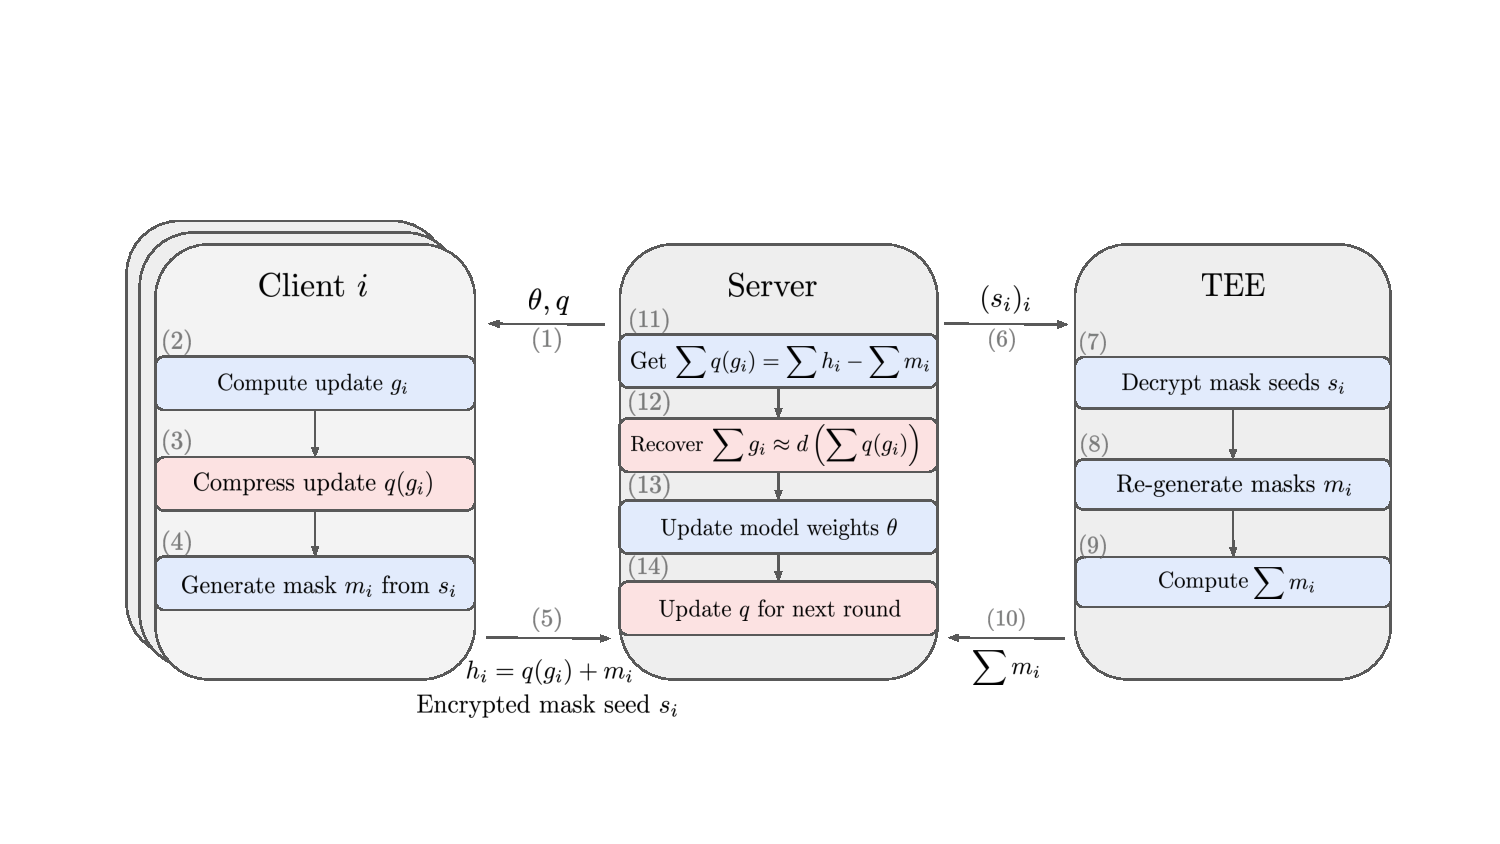
\includegraphics[width=0.8\textwidth]{figs/secagg_summary_new.pdf}
    %\vspace{-5mm}
    \caption{\label{fig:secagg_summary}
    Summary of the proposed approach for one FL round, where we omit the round dependency and \modif{Differential Privacy (DP)} for clarity. Blue boxes denote standard steps and red boxes denote additional steps for uplink compression. Client $i$ computes local model update $g_i$, compresses it with the compression operator $q$, and encrypts it by adding a random mask $m_i$ in the compressed domain, hence reducing the uplink bandwidth (steps 2--4). The server recovers the aggregate in the compressed domain by leveraging any \SecAgg protocol \modif{(steps 7--13, with a TEE-based \SecAgg, see Section~\ref{subsec:secagg})}. Since the decompression operator $d$ is linear, the server can convert the aggregate back to the non-compressed domain, up to compression error (step 12). As with the model weights $\theta$, the compression operator $q$ are also periodically updated and broadcast by the server (step 14). 
    In Section~\ref{sec:method}, we apply the proposed method to scalar quantization and pruning without impacting \SecAgg and propose Secure Indexing, a variant of \SecAgg for extreme uplink compression with product quantization. See Section~\ref{subsec:secagg} for details about \SecAgg and Section~\ref{sec:discussion} for a discussion on~DP.
    }
    \vspace{-3mm}
\end{figure*}



% Our focus in this paper is on 

%Second, scaling cross-device (synchronous) FL to millions of clients with various capabilities and intermittent availability \citep{bonavitz2019federated} suffers from diminishing returns: the wall-clock training time plateaus as the number of clients keeps increasing~\citep{huba2021papaya}. Even though this challenge can be addressed by leveraging the buffered asynchronous aggregation technique proposed by \cite{nguyen2021federated}, compatible with DP and SecAgg, the asynchronous protocol remains bottlenecked by communication latency between the server and the clients.


%Considering the above privacy and scalability goals, we focus on enabling efficient FL communications while keeping a high privacy bar. In addition to the primary objective of speeding up convergence, reducing communication costs brings other significant benefits. Lowering communication requirements addresses selection bias due to undersampling clients with limited connectivity, improving fairness and inclusivity metrics. Better communication efficiency shrinks the carbon footprint of FL, whose fraction attributable to communication can reach 95\%~\citep{qiu2021first}. %Finally, training larger model in FL would be a possibility, when the communication cost is reduced, because local memory or compute requirements can be addressed by modifying the local training loop, for instance with gradient checkpointing \citep{chen2016training}. However, some form of compression would be required to enable efficient communication.


%First, compressing model updates from the client to the server presents several challenges due to compatibility with SecAgg and is an area suitable for further research. 
%Second, upload bandwidth is generally more restricted than download. For instance, according to the most recent FCC report, the ratio of download to upload speeds for DSL/cable providers in the US ranges between 3$\times$ to 20$\times$~\citep{fcc-broadband}. We consider broadband speeds here because devices participate in the FL training while connected to fixed broadband, usually through Wi-Fi~\citep{huba2021papaya}.




% Hence, FL provides the ability to leverage data from massive client populations while ensuring the security and privacy of the client data.
% Go further: compatibility with DP / compression as a mitigation techniques of attacks
% Model and gradient compression intrinsically different.
%  Why not having the secure enclave perform the aggregation?

%\clearpage
\section{Related Work}\label{sec:related}

\noindent{\bf Parallel graph algorithms.}
There are numerous efforts that aim to parallelize generic search schemes on graphs (e.g., BFS~\cite{shun2013ligra}, DFS~\cite{naumov2017parallel}, random walk~\cite{talati2021deep}, beam search~\cite{meister2020best}, and bucketing~\cite{sridhar2019delta,zhang2020optimizing}). However, many of these algorithms were designed without considering having a vector associated with each vertex and a target of achieving high recall under a stringent latency constraint. In contrast, we analyze the search efficiency challenges of ANN and propose optimizations to handle them to allow vector-based similarity search to scale on modern multi-core architectures. Among different algorithms, the most related work to ours is perhaps $\Delta$-stepping~\cite{zhang2020optimizing}, which stages the expansion of nodes in order to avoid redundant expansions. We have applied $\Delta$-stepping to vector search and will provide a more detailed discussion in Section~\ref{subsec:delta-step} and comparison in Section~\ref{sec:eval}.

\noindent{\bf Parallel graph frameworks.}
There has been many graph engines and frameworks developed in the past decade.
Some of them are shared-memory, focusing on processing in-memory datasets within a computation node~\cite{uta2018exploring}, e.g., Galois~\cite{nguyen2013lightweight}, Ligra~\cite{shun2013ligra}, Polymer~\cite{zhang2015numa}, GraphGrind~\cite{sun2017graphgrind}, GraphIt~\cite{zhang2020optimizing}, Graptor~\cite{vandierendonck2020graptor}, and GraphBLAS~\cite{aznaveh2020parallel}.
Some are distributed systems~\cite{rivas2018mpi}, e.g., Pregel \cite{malewicz2010pregel}, GraphLab~\cite{low2014graphlab},  PowerGraph~\cite{joseph2012powergraph}, and Gluon~\cite{dathathri2019gluon}.
Some efforts focus on out-of-core designs (e.g., GraphChi~\cite{aapo2012graphchi} and X-Stream~\cite{roy2013x}) and process large graphs with disk support.
Many graph frameworks are also on GPUs~\cite{DBLP:conf/ppopp/MengLTS19}, such as CuSha~\cite{khorasani2014cusha}, Gunrock~\cite{wang2016gunrock}, GraphReduce~\cite{sengupta2015graphreduce}, Graphie~\cite{han2017graphie}, Multigraph~\cite{hong2017multigraph},  GraphBLAST~\cite{yang2019graphblast}, and Ascetic~\cite{tang2021ascetic}.
These graph systems are either based on a vertex-centric model~\cite{malewicz2010pregel,zhang2018simple} or its variants (e.g., edge-centric~\cite{roy2013x}).
Many of these parallel graph frameworks are designed primarily for generic parallel graph analytics instead of vector-based similarity search. Enabling ANN search in these frameworks, which have matured compilers and optimization technologies, is possible but requires addressing non-trivial portability challenges. For example, the input graphs of existing ANN search can have varying structures, such as hierarchical~\cite{hnsw}, heterogeneous~\cite{diskann,hm-ann}, etc. The search engine also performs additional optimizations such as transaction support~\cite{milvus}, vector reordering, prefetching, and specialized optimizations against different data types, e.g., FP32/INT8. Therefore, porting those changes, to existing frameworks, beyond the search algorithm itself, requires changes across the entire system stack.

\noindent{\bf Heterogeneous memory.}
Heterogeneous memory (HM) is emerging. It combines multiple memory components to construct main memory. HM is typically composed of a high-capacity memory technology such as non-volatile memory (but high memory access latency) and a high-performance memory technology (with limited memory capacity) such as DRAM. 
To make HM performance close to that of DRAM-only, previous work focuses on hardware-~\cite{asplos15:agarwal,hetero_mem_arch,qureshi_micro09, ibm_isca09,gpu_pcm_pact13} and software-based~\cite{eurosys16:dulloor,asplos16:lin,wen:ICS18,sc18:wu,unimem:sc17,luo:NGS,cluster20:ren} solutions to manage data placement on HM. Optane PMM and DRAM are commonly used to build HM. With PMM, the memory capacity on a single machine can achieve 6TB~\cite{optane:ucsd}. However, the latency and bandwidth of PMM is only 1/3 and 1/6 of DRAM. There are two operating modes for PMM, \textit{Memory Mode} and \textit{App-direct Mode}. 
In Memory Mode, DRAM works as a hardware-managed cache to PMM. Running the application in this mode does not require application modifications. App-direct Mode allows the programmer to explicitly control memory accesses to PMM and DRAM. \name works in App-direct Mode and outperforms Memory Mode in billion-scale dataset search (Section~\ref{sec:eval}). 

\section{Method}

Here we discuss the standard retrieve-and-rerank (R\&R) framework for IR (\S{\ref{sec:retrieve_and_rerank}}) and how our proposal fits into it (\S{\ref{sec:cross_encoder_feedback}}). While our approach can be applied to any R\&R framework, we consider a text-based retriever and reranker for simplicity while elaborating our method. A multi-modal R\&R framework is described in \S\ref{sec:multimodal_results}.


\subsection{Retrieve-and-Rerank}
\label{sec:retrieve_and_rerank}
R\&R for IR consists of a first-stage retriever and a second-stage reranker. Modern neural approaches typically use a dual-encoder model as the retriever and a cross-encoder for reranking.  

\paragraph{\textbf{The Retriever}:} The dual-encoder retriever model is based on a Siamese neural network \cite{chicco2021siamese}, containing separate Bert-based \cite{devlin2019bert} encoders $E_Q(.)$ and $E_P(.)$ for the query and the passage, respectively.
Given a query $q$ and a passage $p$, a separate representation is obtained for each, such as the \textsc{cls} output or a pooled representation of the individual token outputs from $E_Q(q)$ and $E_P(p)$. The question-passage similarity $sim(q,p)$ is computed as the dot product of their corresponding representations: query/passage.}
\begin{equation}
    Q_q = Pool(E_Q(q))
\end{equation}
\begin{equation}
    P_p = Pool(E_P(p))
\end{equation}
\begin{equation}\label{eq:sim}
   sim(q,p) = S(Q_q,P_p) = Q_q^TP_p
\end{equation}

Since Eq.~\ref{eq:sim} is decomposable, the representations of all passages in the retrieval corpus can be pre-computed and stored in a dense index \cite{johnson2019billion}. During inference, given a new query, the top $K$ most relevant passages are retrieved from the index via approximate nearest-neighbor search.

\paragraph{\textbf{The Reranker}:} The cross-encoder reranker model uses a Bert-based encoder $E_R(.)$, which takes the query $q$ and a corresponding retrieved passage $p$ together as input and outputs a similarity score. 
A feed-forward layer $F$ is used on top of the \textsc{cls} output from $E_R(.)$ to compute a single logit, which is used as the final reranker score $R(q,p)$. The top $K$ retrieved passages are then ranked based on their corresponding reranker scores.

\begin{equation}
   R(q,p) = F(CLS(E_R(q,p))
\end{equation}


\begin{algorithm}[t]
\caption{\textsc{\textbf{ReFIT}}}
\label{alg4}
\begin{flushleft}
\textbf{Input}: Query $q$ and its representation $Q_q$, retrieved passages $P$ and their representations $\hat{P}$.\newline
\textbf{Output}: Updated query representation $Q_{q,n}$
\end{flushleft}
\begin{algorithmic}[1]
    \State Initialize query vector $Q_{q,0}$ = $Q_q$
    \State Compute reranker distribution $D_{CE}(q,P)$ (Eq.~\ref{eq:d-ce})
    \For{\textit{i in 0 to n}}
        \State Compute retriever distribution $D_{Q_{q,i}}(\hat{P})$ (Eq.~\ref{eq:d-q})
        \State Compute loss $\mathcal{L}$ (Eq.~\ref{eq:loss})
        \State Update $Q_{q,i+1} = Q_{q,i} - \alpha \frac{\partial}{\partial Q_{q,i}}\mathcal{L}$
    \EndFor
    \State return $Q_{q,n}$
\end{algorithmic}
%\vspace{-0.4em}
\end{algorithm}

\subsection{Reranker Relevance Feedback}
\label{sec:cross_encoder_feedback}
The main idea underlying our proposal is to compute an improved query representation for the retriever using feedback from the more powerful reranker.
More specifically, we perform a lightweight inference-time distillation of the reranker's knowledge into a new query vector.

Given an input query $q$ during inference, we use the following output provided by the R\&R pipeline:
\begin{itemize}
   \item Query representation $Q_q$ from the retriever.
    \item Retrieved passages $P = \{p_1, p_2,  ..., p_K\}$ and their representations $\hat{P} = [P_{p_1}, P_{p_1},  ..., P_{p_K}]$ from the retriever. 
    \item The reranking scores $R(q,P) = [R(q,p_1),..., R(q,p_K)]$.
\end{itemize}
Note that $\hat{P}$ above is directly obtained from the passage index and is not computed during inference.

The proposed reranker feedback mechanism begins with using the reranking scores $R(q,P)$ to compute a cross-encoder ranking distribution $D_{CE}(q,P)$ over passages $P$ as follows:

\begin{equation}
D_{CE}(q,P)=\mathrm{softmax}([R(q,p_1), ..., R(q,p_K)])
\label{eq:d-ce}
\end{equation} 

The query and passage representations from the retriever are used to compute a similar distribution $D_{Q_q}(\hat{P})$ over $P$:

\begin{equation}
    D_{Q_q}(\hat{P}) = \mathrm{softmax}([Q_q^TP_{p_1}, ..., Q_q^TP_{p_K}])
    \label{eq:d-q}
\end{equation}

Next, we compute the loss as the KL-divergence between the retriever and reranker distributions:

\begin{equation}
    \mathcal{L} = D_{KL}(D_{CE}(q,P) || D_{Q_q}(\hat{P}))
    \label{eq:loss}
\end{equation}

which is then used to update the query vector via gradient descent. The query vector update process is repeated for $n$ times, where $n$ is a hyper-parameter. 
A schematic description of the process can be found in Algorithm \ref{alg4}. 

Finally, the updated query vector $Q_{q,n}$ is used for a second-stage retrieval from the passage index.  
From dual-encoder retrieval with the updated $Q_{q,n}$, we aim to achieve better recall than with the initial $Q_q$, while obtaining a ranking performance that is comparable with that of the reranker.








%!TEX root = ../main.tex
\section{Experiments}
\label{sec:exp}

We conduct preliminary experiments to demonstrate the effectiveness of \sys. 
We evaluate its performance in two key processes: Reasoning and Verification. %The multimodal data lakes and data discovery techniques used in these experiments are discussed respectively for each process. 

%\subsection{Question Answering using Retrieved Multimodal Data}

%To validate the effectiveness of our method in text reasoning and mutimodal (text+image) reasoning, we design the experiment on natural language question answering and visual-based entity question answering.

\subsection{Question Answering}

\stitle{Experiment Setting.} In this experiment, we focus on evaluating question answering performance using a multimodal data lake consisting of 400K web tables and 6M English passages extracted from Wikipedia. The data lake includes both tables and texts, and each query is designed to retrieve relevant data items to answer a given question. We use 18 manually crafted user queries, each with corresponding ground truth annotations specifying the required data items, sub-queries for decomposition, and final answers.

\stitle{Data Discovery Evaluation.}
The effectiveness of data discovery is measured using the recall at $K$ (R@$K$) metric, which calculates the proportion of relevant data items retrieved in the top-$K$ recommendations. The experimental results show that when $K$ is 5, 10, 15, and 20, the R@$K$ values are 40.8\%, 46.3\%, 59.3\%, and 77.8\%, respectively. For 12 out of the 18 queries, \sys successfully discovers all the relevant items needed to answer the query. The remaining 6 queries show partial success. In total, 30 out of 38 related items are correctly discovered, demonstrating the potential of the proposed data discovery methodology, even though it is still in a preliminary stage.


\stitle{Query Decomposition Evaluation.}
To decompose queries into manageable sub-queries, \sys serializes the discovered data items and uses GPT-3 to generate sub-queries. The output includes the sub-queries and corresponding data item ids. Evaluation of the decomposition quality is based on two criteria: (1) whether each sub-query is useful for solving the original query, and (2) whether the sub-query can be answered correctly using the selected data item. The human evaluation results show that 77.8\% of the queries scored 2 (both criteria met), 16.7\% scored 1 (only the first criterion met), and 5.5\% scored 0. 

Table~\ref{tab:results_of_decomposition} shows the results of 8 instances. \sys is able to handle different aggregation operations, such as sum (Instance 2) and comparison (Instance 3). Further, it correctly understands long sentences (Instance 1). However, \sys has difficulty in dealing with sentences with complex syntactic structures (\eg in Instance 4, GPT-3 mistakenly generates $q_3$ because it takes the subject of released'' as Academy Award for Best Foreign Language Film''.). 


\begin{table}[!t]
\centering
\resizebox{\textwidth}{!}{
{\small
\begin{tabular}{p{15cm}}
\hline
\underline{Instance 1}: $Q$: Did the 2014 United States house of representatives elections take place on the same day in Rhode Island, South Carolina and Louisiana? $E = \{P_1, P_2, P_3\}$\\
$\rightarrow$ $q_1$: Did the 2014 United States House of Representatives elections take place on November 4, 2014 in Rhode Island? $e_1 = P_1$; $q_2$: Did the 2014 United States House of Representatives elections take place on November 4, 2014 in South Carolina? $e_2 = P_2$; $q_3$: Did the 2014 United States House of Representatives elections take place on November 4, 2014 in Louisiana? $e_3 = P_3$ \\
$\bigstar$ Score: 2 \\
\hline
\underline{Instance 2}: $Q$: How many representatives were elected in the 2014 United States house of representatives elections in Rhode Island and South Carolina?   %\srm{Question is vague, are we asking for a sum?}
$E = \{P_1, P_2\}$ \\
$\rightarrow$ $q_1$: How many representatives were elected in the 2014 United States house of representatives elections in Rhode Island? $e_1 = P_1$; $q_2$: How many representatives were elected in the 2014 United States house of representatives elections in South Carolina? $e_2 = P_2$ \\
$\bigstar$ Score: 2 \\
\hline
\underline{Instance 3}: $Q$: Which number is larger, the number of living former prime ministers of Tunisia or the number of former presidents of Ghana? $E = \{T_1, P_1\}$ \\
$\rightarrow$ $q_1$: What is the number of living former prime ministers of Tunisia? $e_1 = P_1$; $q_2$: What is the number of former presidents of Ghana? $e_2 = T_1$ \\
$\bigstar$ Score: 2 \\
\hline
\underline{Instance 4}: $Q$: What year was the first German film that won the Academy Award for Best Foreign Language Film released? $E = \{T_1, P_1\}$ \\
$\rightarrow$ $q_1$: What year was the film The Tin Drum released? $e_1 = T_1$; $q_2$: What was the first German film that won the Academy Award for Best Foreign Language Film? $e_2 = T_1$; $q_3$: What year was the first Academy Award for Best Foreign Language Film given out? $e_3 = T_1$ \\
$\bigstar$ Score: 0 \\
\hline
\underline{Instance 5}: $Q$: Did The Tin Drum and Kolya both win the Academy Awards for Best Foreign Language Film? $E = \{P_1, P_2\}$ \\
$\rightarrow$ $q_1$: whether The Tin Drum has ever won the Academy Award for Best Foreign Language Film? $e_1 = P_1$; $q_2$: whether Kolya has ever won the Academy Award for Best Foreign Language Film? $e_2 = P_2$ \\
$\bigstar$ Score: 2 \\
\hline
\underline{Instance 6}: $Q$: How many years elapsed between the premiere of season 10 and the premiere of season 5 of Law \& Order : Special Victims Unit? $E = \{T_1, T_2\}$ \\
$\rightarrow$ $q_1$: What is the premiere date of season 10 of Law \& Order : Special Victims Unit? $e_1 = T_2$; $q_2$: What is the premiere date of season 5 of Law \& Order : Special Victims Unit? $e_1 = T_1$ \\
$\bigstar$ Score: 2 \\
\hline
\underline{Instance 7}: $Q$: Did You Let Me Walk Alone participate in the Eurovision Song Contest in 1996? $E = \{T_1, P_1\}$ \\
$\rightarrow$ $q_1$: What year was the Eurovision Song Contest held in Lisbon, Portugal? $e_1 = T_1$; $q_2$: What year was You Let Me Walk Alone released? $e_2 = P_1$ \\
$\bigstar$ Score: 1 \\
\hline
\underline{Instance 8}: $Q$: Are the tallest building in the united kingdom and the tallest building in poland above 200 meters? $E = \{T_1, T_2\}$\\
$\rightarrow$ $q_1$: What is the height of the tallest building in the United Kingdom? $e_1 = T_1$; $q_2$: What is the height of the tallest building in Poland? $e_2 = T_2$ \\
$\bigstar$ Score: 2 \\
\hline
\end{tabular}
}
}
\caption{Example sub-queries generated by \sys. $q_i$ and $e_i$ represent the $i_{th}$ sub-query and its corresponding data item. $T_i$ represents a table and $P_i$ represents a text. 
}
\label{tab:results_of_decomposition}
\end{table}


% \subsubsection{Visual-based Entity Question Answering}

% \stitle{Experiment Setting.}
% The experiments were conducted in a zero-shot setting using RTX 4090 GPUs. For GPT-4V, we used the interface of the GPT-4-vision-preview model. It's worth noting that GPT-4V often refrains from answering person identify questions without additional clues due to policy reasons. However, with the incorporation of matching graph techniques, it can leverage weak signals and combine them with its own knowledge base. For the dataset, we chose NewsPersonQA~\cite{zhang2024mar}. For the task evaluation, we use accuracy (\textbf{Acc}) as an evaluation metric. Furthermore, we assess the accuracy only for instances where relevant clues are successfully retrieved, which is denoted as \textbf{Acc}$^{{hit}}$.

% \stitle{Baseline.} For answering queries, we selected two well-known and highly capable MLLMs, as well as human evaluation,to serve as baselines. \textbf{LLaVA:} 
% This model utilizes CLIP-ViT-L-336px with an MLP projection. We refer to the 1.5 version with 7 billion parameters as LLaVA-7b and the version with 13 billion parameters as LLaVA-13b.
% \textbf{GPT-4V:} 
% Recognized as OpenAI's most powerful general-purpose MLLM to date, GPT-4V boasts 1.37 trillion parameters. 

% \stitle{Main Results.} The main results of visual-based entity question answering are summarized in Table~\ref{tbl:single}, which leads to the following insights: LLaVA-13b demonstrates higher accuracy (27.93\%) compared to LLaVA-7b (22.26\%), suggesting that a model's recognition ability is positively correlated with its parameter size, which to some extent reflects its knowledge base. Incorporating a matching graph leads to an 8.9\% improvement in accuracy for LLaVA-7b and a 3.2\% improvement for LLaVA-13b. GPT-4V, with matching, achieves a character recognition accuracy of 34.83\%.
%  The enhancement from matching is more pronounced for LLaVA-7b than for LLaVA-13b, indicating that while matching can compensate for differences in parameters, a model's inherent capabilities still set an upper limit on its performance.

% \begin{table}[t!]
% \caption{Result for Visual-based Entity Question Answering. (Note: GPT-4V could not answer these queries directly due to policy constraints. Values within parentheses are those GPT-4V still refuses to answer.)}
% \small
% \centering
% \label{tbl:single}
% \resizebox{0.5\columnwidth}{!}{
% \begin{tabular}{l|l|l}
% \toprule
% {\textbf{Models}}     & \textbf{Acc} (\%) & \textbf{Acc}$^{{hit}}$ (\%) \\ 
% \midrule
% \textbf{LLaVA-7b}                        & 22.26        & 27.53         \\
% {\textbf{LLaVA-7b + Symphony}} & 31.19        & 62.81         \\ 
% \hline
% \textbf{LLaVA-13b}                       & 27.93        & 32.86         \\
% {\textbf{LLaVA-13b + Symphony}} & 31.13        & 62.34         \\ 
% \hline
% \textbf{GPT-4V}                          & -            & -             \\
% {\textbf{GPT-4V + Symphony}} & 34.84 (4.2)  & 68.31 (2.6)  \\ 
% \midrule
% \textbf{Symphony(Graph Reasoning)}                            & {\bf 39.09}        & {\bf 79.65}         \\ 
% \bottomrule
% \end{tabular}
% }
% \end{table}


\subsection{Answer Verification}

We showcase preliminary experimental results that highlight the initial achievements of \sys in facilitating the verification of generative AI. 
% \yang{Do we need to include tuple-tuple and text generation?}

\stitle{Experiment Setting.}
We perform a controlled study to assess textual claims, employing 1,300 textual claims from the TabFact~\cite{chen2019tabfact} benchmark, which is currently the most advanced benchmark for verifying the credibility of textual hypotheses by utilizing a given table. The data lake consists of 16,573 tables from the TabFact and 2,925 tables sourced from WikiTable-TURL~\cite{deng2022turl}.


\begin{figure}[t!]
\vspace{1em}
\begin{center}
  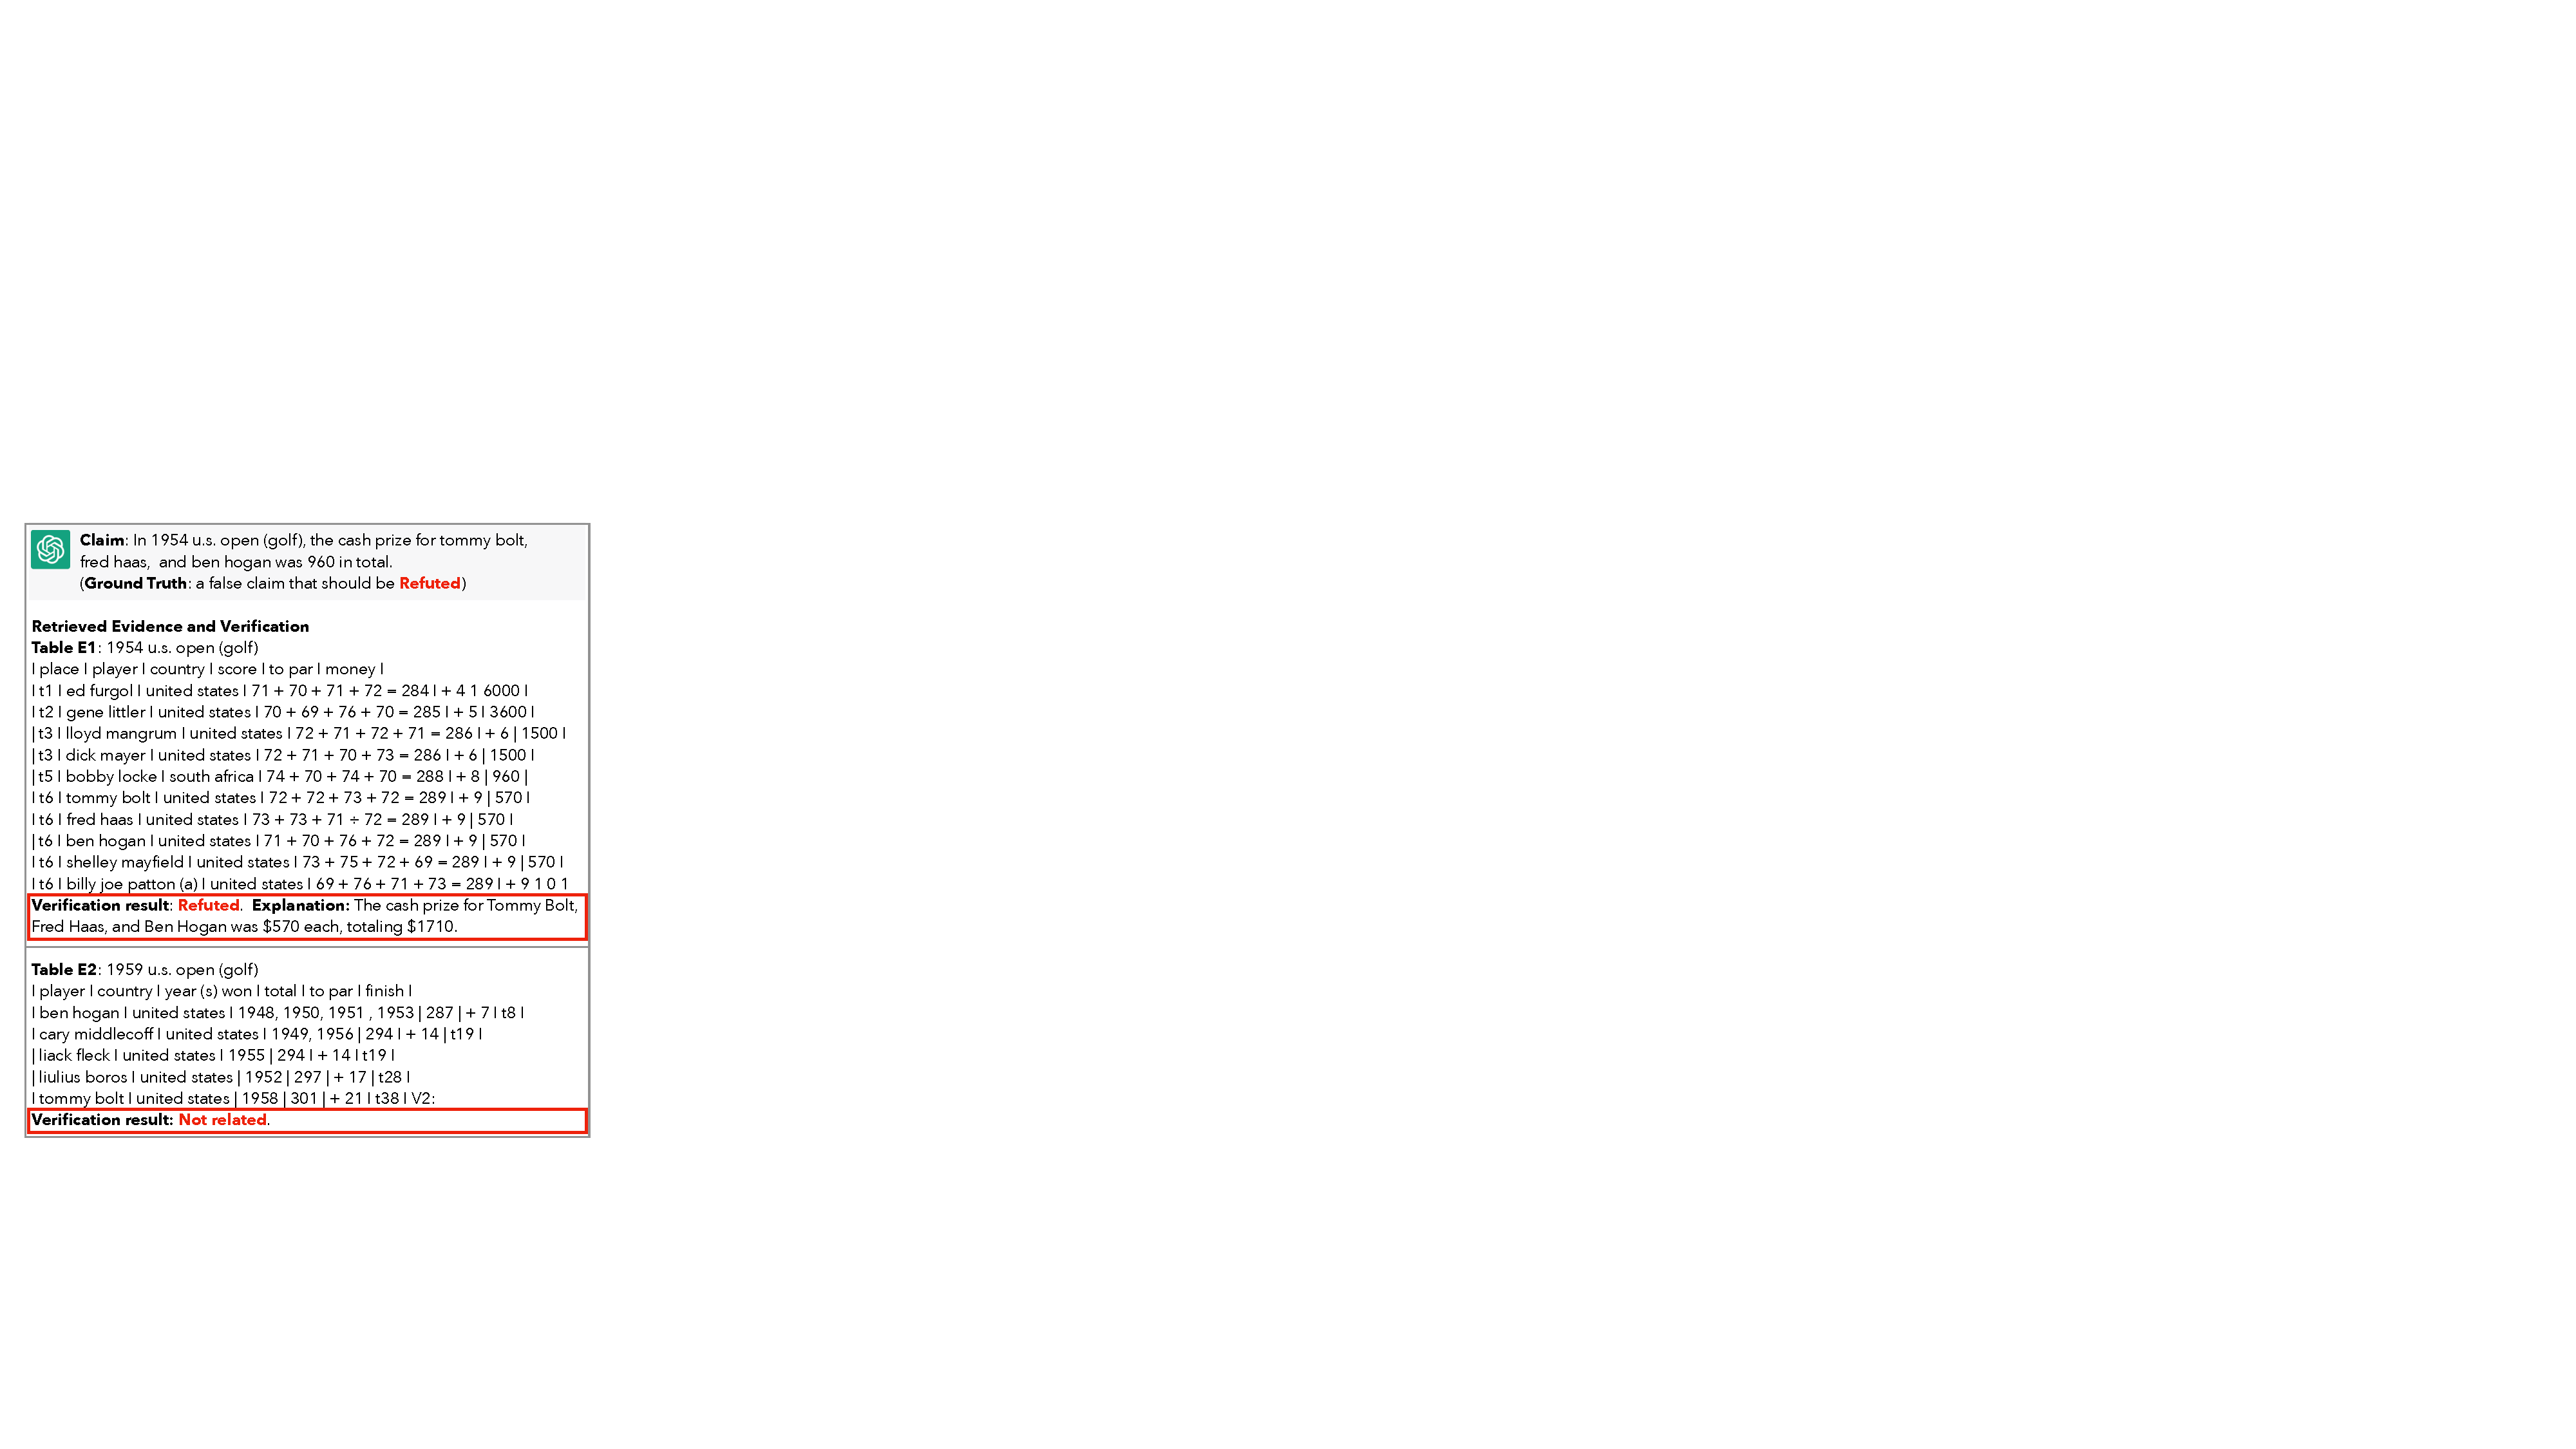
\includegraphics[width=0.65\textwidth]{submissions/Nan2024/figs/tabfact.pdf}
  \caption{Verifying a textual claim using retrieved tables.}
  \label{fig:claim_case} 
\end{center}
\end{figure}


\stitle{Evaluation for Retrieval.} 
We use Elasticsearch~\cite{elasticsearch} to retrieve the top-5 tables for each textual claim. Given the limited amount of relevant data, we focus on the recall metric for evaluation. Each textual claim is associated with a corresponding table in the original dataset, which we consider relevant evidence, while other retrieved tables are deemed irrelevant. The retrieval performance, measured by R@5, is 0.88.

\stitle{Evaluation for Verification.} 
We evaluate the verification process using two different verifiers: GPT-3.5, the default verifier for both data types, and PASTA~\cite{pasta}, a specialized model for text verification.
%
The performance of the verifiers is measured by accuracy. When the retrieved data cannot support or refute a claim, the verifier outputs ``not related''. However, in this case, since PASTA that only offers two different answers: ``true'' or ``false'', we consider it's also correct when PASTA outputs ``false''.

We conduct experiments in two settings. When a relevant table is retrieved and provided as evidence to the verifier, PASTA achieves higher accuracy than GPT-3.5 (0.89 vs. 0.75) in verifying the textual claim based on the table. However, in cases where many of the retrieved tables are irrelevant to the claim, the verifier must accurately determine which tables are not related. In this setting, PASTA's accuracy drops to 0.72 because it has not encountered this scenario during training, while GPT-3.5 improves to 0.91. 
% Thus, GPT-3.5-turbo demonstrates superior generalization capabilities and performs better than PASTA when dealing with irrelevant tables.
Thus, when the retrieved data is highly related to the generative data, local models like PASTA have higher accuracy while protecting privacy. In contrast, GPT-3.5 is better at generalizing and providing explanations for further judgments. Users can select the appropriate model based on their requirements.


In Figure~\ref{fig:claim_case}, we present a case of verifying a textual claim based on retrieved tables using GPT-3.5. \sys retrieves two tables $E_1$ and $E_2$, where $E_1$ can be used with an aggregation query to refute the claim while $E_2$ is not related because it is for the year 1959. The red boxes in Figure~\ref{fig:claim_case} show that GPT-3.5 can provide not only a verification result but also some explanation.






\section{Conclusion and Future Work}
We demonstrate that query representations can be improved using feedback from a cross-encoder reranker \textit{at inference time} for better performance of dual-encoder retrieval. This work proposes for distillation using relevance feedback from the reranker as a better and faster alternative to the traditional strategy of reranking a larger pool of candidates for improving recall.
\textsc{ReFIT} is lightweight and improves retrieval accuracy across different domains, languages and modalities over a state-of-the-art retrieve-and-rerank pipeline with comparable latency. Future work will focus on the potential integration of textual relevance feedback from large language models (LLMs). Additionally, a promising area of exploration lies in enhancing the interpretability by examining how relevance feedback influences the significance of individual query terms within the query representation.


\section{Limitations}

\textsc{ReFIT} introduces an additional latency into a traditional retrieve-and-rerank framework.
The distillation time is only dependent on the number of updates, and is unaffected by the model architecture  and number of retrieved passages; the overall additional latency (as per Table \ref{tab:inf_times}) amounts to an extra 17.5\% on GPU (or 4.4\% on CPU) when the number of retrieved passages $K$=100. However, it is noteworthy that \textsc{ReFIT} remains faster and exhibits superior performance compared to the standard approach of reranking a larger pool of candidates for improving recall.
Moreover, the efficacy of our approach is contingent upon the reranker providing a better ranking than the retriever. We anticipate that our method might provide minimal gains in situations where the retriever performs similar to the reranker.

\bibliographystyle{ieeetr}

\bibliography{submissions/Revanth2024/sample-base}

\end{document}
